\section{Despesas}

As despesas inerentes ao presente projeto encontram-se intrincadamente associadas a três fontes de destaque, nomeadamente: infraestrutura, recursos humanos e angariação de clientes.

\subsection{Infraestrutura}

Os ônus relativos à infraestrutura do projeto serão integralmente derivados dos serviços providos pela plataforma \textit{\gls{Azure}}, visto que as demais instâncias participantes se pautam pela isenção de custos. A delimitação do preço desses serviços foi efetuada por intermédio da aplicação da Calculadora de Custos \textit{\gls{AzurePricingCalculator}}. Nesse processo de cálculo, foram criteriosamente incorporados os serviços de \textit{\gls{AppService}} e \textit{\gls{AzureSQLDatabase}}, a fim de mensurar com precisão os dispêndios vinculados a tais soluções. A tabela \ref{estimativaAzure} elucida a projeção orçamentária referente à Azure.

\begin{table}[H]
    \setcounter{table}{0}
    \center
	\caption{Custos Azure Services}
    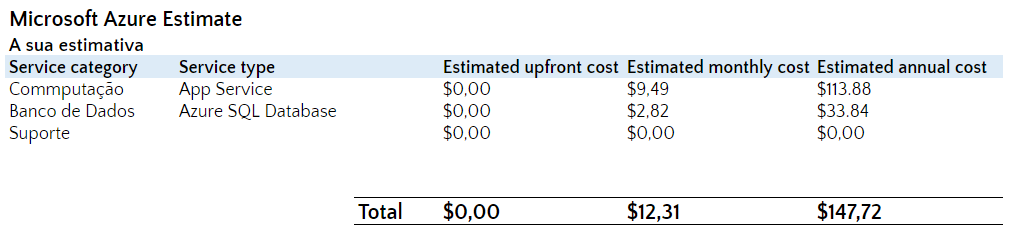
\includegraphics[scale=0.55]{imagens/viabilidadeFinanceira/estimativaAzure.png}
    \label{estimativaAzure}
	\fonte{Azure Pricing Calculator}
\end{table}

De acordo com a estimativa de usuários realizada, foi possível estimar também os custos de infraestrutura gerados, fornecendo uma visualização dessa fonte de despesas, como pode ser visto na tabela \ref{estimativaAzure}.

\subsection{Recursos Humanos}

No contexto de um projeto no âmbito da tecnologia, a apropriação dos recursos financeiros destinados aos elementos humanos compreende uma amplitude abrangente de fatores mutuamente interligados. Estes englobam componentes como a remuneração dos colaboradores, as obrigações fiscais e previdenciárias, as vantagens e benefícios oferecidos, as iniciativas de aperfeiçoamento e o contínuo desenvolvimento profissional. A competente gestão desses recursos assume um papel preponderante, exercendo uma influência crucial no sucesso do empreendimento e na maximização dos aportes investidos.

No que tange às remunerações, os desembolsos podem variar significativamente devido às posições ocupadas e ao nível de especialização dos membros da equipe. Os encargos trabalhistas, abarcando as contribuições sociais e outras obrigações jurídicas, também compõem a soma total dedicada.

A concessão de benefícios, como planos de saúde, auxílios-alimentação e transporte, se converte em um elemento adicional, conferindo um acréscimo financeiro ao montante designado. A capacitação da equipe, mediante a implementação de programas de formação e atualização, insere-se no âmbito do investimento, salvaguardando a manutenção da excelência laboral em um cenário tecnológico em constante mutação.

De acordo com as orientações preconizadas por plataformas especializadas em oportunidades de trabalho, análises de mercado e organizações dedicadas ao recrutamento, os valores correspondentes às despesas podem ser delineados com base em uma média geral:

\begin{itemize}
    \item \textbf{Salário de Estágio}: R\$ 1.500,00;
    \item \textbf{Encargos Trabalhistas (aproximadamente 70\% do salário)}: R\$ 1.050,00;
    \item \textbf{Benefícios (plano de saúde, vale-transporte, vale-alimentação)}: R\$ 300,00.
\end{itemize}

Considerando que a configuração da equipe é constituída por um grupo de seis desenvolvedores em nível de estágio, os montantes financeiros mensais que imperam no cenário comercial foram incorporados à análise, conforme o Quadro \ref{despesasRecursosHumanos}:

\begin{itemize}
    \item Custo base: R\$ 2.800,00
    \item Dias-base: 22 | Dia-hora: 8
    \item Custo-hora: R\$ 15,90
\end{itemize}

\begin{quadro}[H]
\centering
\caption{Despesas dos Recursos Humanos}
\label{despesasRecursosHumanos}
\begin{longtable}{|p{5cm}|p{3cm}|p{3cm}|}
\hline
Despesa & 6 meses & 12 meses
\\\hline
Salário & R\$ 54.000,00 & R\$ 108.000,00\
\\\hline
Encargos Trabalhistas & R\$ 37.800,00 & R\$ 75.600,00\
\\\hline
Benefícios & R\$ 10.800,00 & R\$ 21.600,00\
\\\hline
\end{longtable}
\fonte{Os Autores.}
\end{quadro}

A contabilização das horas referentes ao projeto incorporou a análise de três distintas classificações de requisitos funcionais a serem incorporados: níveis fácil, médio e difícil, organizados em conformidade com a proficiência dos membros da equipe.

Para os requisitos funcionais fáceis, foi tomado como base um tempo de 48 horas de desenvolvimento. Já para os médios foi considerado o tempo de 80 horas de desenvolvimento e, para os difíceis, 160 horas. Tais despesas desempenham um papel preponderante especialmente ao longo da fase de desenvolvimento do projeto. A representação gráfica \ref{maoDeObra} evidencia a apresentação destes cálculos.

\begin{table}[H]
    \center
    \setcounter{table}{1}
	\caption{Mão de Obra Mensal}
    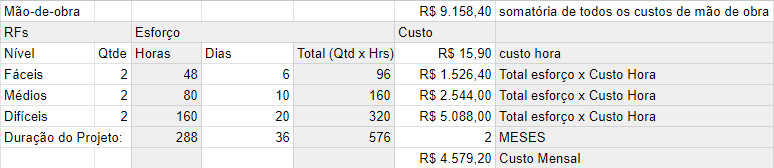
\includegraphics[scale=0.75]{imagens/viabilidadeFinanceira/MaoDeObra.png}
    \label{maoDeObra}
	\fonte{Os autores}
    \setcounter{table}{2}
\end{table}

A tabela \ref{maoDeObra} demonstra a quantidade de horas totais a serem utilizadas no projeto, bem como os custos totais com mão de obra e os custos mensais a serem assumidos. De acordo com o cálculo de horas realizado na tabela, é possível observar que a duração será de 2 meses.

\subsection{Captação de Clientes}

Com vistas a consolidar a estratégia de aquisição de clientes para a plataforma, almeja-se direcionar recursos para atividades de marketing. Isso se concretizará mediante a veiculação de anúncios em plataformas conexas ao público-alvo do projeto, a exemplo do \textit{\gls{Youtube}}, \textit{\gls{Twitch}} e \textit{\gls{Tiktok}}. A ênfase recairá na promoção desses anúncios em conteúdos especialmente voltados ao universo dos jogos eletrônicos, visando estabelecer uma afinidade precisa e maximizar a eficácia das iniciativas na atração de novos usuários para a \textit{GameLocker}.

Ademais, uma possibilidade viável consiste na divulgação nestas plataformas mediante um enfoque mais personalizado, alcançado por meio do estabelecimento de colaborações diretas com os criadores de conteúdo. A concretização destas parcerias seria intermediada por acordos de patrocínio, nos quais eles divulgariam o sistema perante sua audiência.

Dentro do contexto de cada uma das mencionadas plataformas, que permitem valores personalizados de investimento em marketing, estima-se, em um primeiro momento, um aporte de investimento mensal equivalente a R\$ 267,00, culminando, assim, em um montante total de R\$ 800,00 mensais destinado à angariação de novos usuários. Estes valores têm o objetivo de manter a captação de usuários ativa sem que o projeto se torne inviável financeiramente.